\documentclass{article}
\usepackage[utf8]{inputenc}
\usepackage[polish]{babel}
\usepackage[T1]{fontenc}
\usepackage{graphicx}
\usepackage{float}
\usepackage[a4paper, left=3.7cm, right=3.7cm, top=3cm, bottom=2cm]{geometry}

\title{Projekt PAM - aplikacja służąca do rozwiązywania testów}
\author{Antoni Załupka}

\begin{document}
	\thispagestyle{empty}
	
	
	\vspace{4cm}
	
	\rule{\linewidth}{2mm} 
	
	\begin{center}
		\huge \textbf{Projektowanie Webowych Aplikacji Graficznych} \\
		\huge {Aplikacja webowa służąca do rozwiązywania testów} \\
	\end{center}
	
	\rule{\linewidth}{0.5mm} 
	
	\vspace{2cm}
	
	\begin{center}
		\Large{Antoni Załupka} \\
		\Large{Numer indeksu: 351120} \\
		\Large{III rok, grupa PAW2} \\
		
	\end{center}
	
	
	\vspace{14cm}
	
	\begin{center}
		\Large{2025, Uniwersytet Śląski}
	\end{center}
	
	\newpage
	
	\tableofcontents
	
	\newpage
	
	\section{Wstęp}
	Celem niniejszego projektu było zaprojektowanie oraz zaimplementowanie edukacyjnej aplikacji webowej w formie quizów stworzonej z wykorzystaniem technologii Vue. Aplikacja ma też uproszczoną wersję mobilną. 
	
	Quizy dostępne w aplikacji nie służą wyłącznie weryfikacji wiedzy użytkownika, lecz pełnią funkcję edukacyjną. Każde pytanie umożliwia niezwłoczne sprawdzenie poprawności odpowiedzi oraz jej modyfikację, co umożliwia naukę w oparciu o szybką informację zwrotną.

    \section{Założenia}
    Aplikacja została stworzona symultanicznie z wersją mobilną. 
        Wersja mobilna jest uproszczona i została napisana w technologii Flutter.
        Obie aplikacje korzystają z tego samego API. 
        API wykonałem w technologii GraphQL, co pozwoliło na elastyczne pobieranie danych i minimalizację liczby zapytań.
        Część serwerową oraz przeglądarkową napisałem w języku TypeScript, co zapewniło lepszą kontrolę typów i ułatwiło rozwój projektu.
        W dalszej części sprawozdania skupię się na przeglądarkowej części projektu, ponieważ jej dotyczy moduł.

    \subsection{Wymagania funkcjonalne}
	\begin{itemize}
		\item Możliwość logowania do aplikacji;
		\item Pobieranie danych z API, w tym quizów oraz historii podejść użytkownika;
		\item Rozwiązywanie quizów i natychmiastowe, asynchroniczne zapisywanie postępu;
		\item Przeglądanie historii podejść w dedykowanej zakładce;
		\item Możliwość edycji, usunięcia i wylogowania się z konta.
	\end{itemize}
	
	\subsection{Wymagania niefunkcjonalne}
	\begin{itemize}
		\item Intuicyjny i przejrzysty interfejs użytkownika;
		\item Wysoka responsywność aplikacji na różnych urządzeniach;
		\item Bezpieczna obsługa danych użytkownika (autoryzacja poprzez token JWT);
		\item Wydajna komunikacja z API (minimalizacja liczby zapytań);
		\item Utrzymanie spójności z wersją mobilną aplikacji.
	\end{itemize}

    \section{Wykorzystane technologie}
        \subsection{Backend}
        \begin{itemize}
            \item Interpreter JavaScript Node.js
            \item Framework Express
            \item Komunikacja GraphQL -- Apollo Server 
            \item Baza danych SQLite
        \end{itemize}
        \subsection{Frontend}
        \begin{itemize}
            \item Vite - szybki bundler i serwer deweloperski
            \item Vue.js - framework do budowy interfejsu
            \item Pinia - zarządzanie stanem aplikacji
            \item Shadcn - biblioteka komponentów UI
            \item Apollo Client - komunikacja z API GraphQL
            \item Vue Router - zarządzanie trasami aplikacji
            \item Tailwind CSS - framework CSS do stylizacji za pomocą klas
        \end{itemize}

    \section{Struktura projektu}
    \begin{itemize}
      \item \textbf{frontend/}
      \begin{itemize}
        \item \textbf{public/}
        \begin{itemize}
          \item \textbf{index.html} – główny plik HTML aplikacji
        \end{itemize}
        \item \textbf{src/}
        \begin{itemize}
          \item \textbf{main.ts} – punkt wejścia Vue, inicjalizacja Pinia i routera
          \item \textbf{App.vue} – główny komponent aplikacji
          \item \textbf{router.ts} – konfiguracja tras (vue-router)
          \item \textbf{apollo-client.ts} – konfiguracja klienta GraphQL (Apollo)
          \item \textbf{style.css} – globalne style CSS i zmienne koloru
          \item \textbf{vite.config.ts} – konfiguracja bundlera i serwera deweloperskiego (Vite)
          \item \textbf{vite-env.d.ts} – definicje typów dla Vite
          \item \textbf{components/} – komponenty UI (ui/, Header/, itp.)
          \item \textbf{pages/} – widoki i strony routowane
          \item \textbf{stores/} – magazyny stanów (Pinia: userStore, attemptStore)
          \item \textbf{services/} – usługi komunikacji z API (quizService, aiService, itp.)
          \item \textbf{lib/} – funkcje pomocnicze (utils.ts)
        \end{itemize}
        \item \textbf{package.json}, \textbf{tsconfig.json}, \textbf{README.md}
      \end{itemize}
    \end{itemize}

    \section{Zarządzanie stanem aplikacji}
      Aplikacja wykorzystuje Pinia jako magazyn stanu. Pinia jest nowoczesnym rozwiązaniem do zarządzania stanem w Vue, które stopniowo zastępuje Vuex. Poniżej przedstawiam dwa główne magazyny stanu.

      \subsection{Pinia Store: \texttt{useUserStore}}
      \label{sec:userStore}
      
      Store \texttt{useUserStore} odpowiada za zarządzanie stanem uwierzytelnionego użytkownika oraz procesami logowania i wylogowania. Główne elementy tego store’u:
      
      \begin{itemize}
        \item \textbf{Stany (ref):}
          \begin{itemize}
            \item \texttt{user: User | null} – przechowuje dane zalogowanego użytkownika.
            \item \texttt{isLoading: boolean} – flaga statusu ładowania podczas wywoływania akcji.
            \item \texttt{error: string | null} – komunikat błędu w przypadku niepowodzenia akcji.
          \end{itemize}
      
        \item \textbf{Akcje:}
          \begin{itemize}
            \item \texttt{async login(email, password)} – wywołuje \texttt{userService.login}, ustawia \texttt{user} i obsługuje błędy.
            \item \texttt{async logout()} – wywołuje \texttt{userService.logout}, czyści \texttt{user}.
            \item \texttt{async loadUser()} – pobiera bieżące dane użytkownika przez \texttt{userService.getMe}, w razie braku uwierzytelnienia przekierowuje na stronę logowania, w przeciwnym razie do listy quizów.
          \end{itemize}
      
        \item \textbf{Integracja z routerem:}
          \begin{itemize}
            \item Store wykorzystuje \texttt{useRouter} do nawigacji (\texttt{/auth/login} lub \texttt{/quizzes}) w zależności od rezultatu sprawdzenia, czy użytkownik po włączeniu strony jest zalogowany.
          \end{itemize}
      \end{itemize}
      
      Dzięki temu store centralizuje logikę uwierzytelniania, obsługi błędów oraz przekierowań, co ułatwia zarządzanie stanem sesji użytkownika w całej aplikacji.  

    \subsection{Pinia Store: \texttt{useAttemptStore}}
      \label{sec:attemptStore}

      Store \texttt{useAttemptStore} odpowiada za zarządzanie stanem pojedynczego podejścia do quizu oraz za mierzenie czasu trwania sesji. Poniżej główne elementy tego store’u:

      \begin{itemize}
        \item \textbf{Stany (ref):}
          \begin{itemize}
            \item \texttt{attempt: QuizAttempt | null} – aktualne podejście (ID, wynik, pytania itp.).
            \item \texttt{quiz: Quiz | null} – metadane quizu (tytuł, opis).
            \item \texttt{questions: Question[]} – lista pytań dla danego podejścia.
            \item \texttt{sessionTime: number} – odliczany w sekundach czas trwania podejścia.
            \item \texttt{intervalId: number | null} – identyfikator timera używanego do odmierzania czasu sesji.
          \end{itemize}

        \item \textbf{Akcje:}
          \begin{itemize}
            \item \texttt{set(newAttempt)} – inicjalizuje nowe podejście i zeruje licznik czasu.
            \item \texttt{update()} – asynchronicznie pobiera najświeższe dane podejścia z serwisu backendowego.
          \end{itemize}

        \item \textbf{Computed:}
          \begin{itemize}
          	\item \texttt{score} – procentowy wynik podejścia, liczony jako:
          	\[
          	\mathrm{round}\left(\frac{\texttt{correctAnswers}}{\texttt{questions.length}} \times 100\right)
          	\]
          \end{itemize}

        \item \textbf{Watchery:}
          \begin{itemize}
            \item Po każdej zmianie \texttt{attempt.value} store automatycznie ładuje:
              \begin{itemize}
                \item metadane quizu przez \texttt{quizService.getQuiz}
                \item listę pytań przez \texttt{questionService.getQuestions}
              \end{itemize}
          \end{itemize}

        \item \textbf{Lifecycle hooks:}
          \begin{itemize}
            \item \texttt{onMounted} – uruchamia timer (co sekundę inkrementuje \texttt{sessionTime}).
            \item \texttt{onUnmounted} – czyści timer, by nie zostawić wiszących interwałów.
          \end{itemize}
      \end{itemize}

      Dzięki takiej strukturze store izoluje logikę pobierania i przetwarzania danych podejścia, a także zarządza pomiarem czasu trwania sesji quizowej.

      \section{Interfejs użytkownika i system komponentów}
      Aplikacja została zbudowana z wykorzystaniem modułowego systemu komponentów, co pozwoliło na zachowanie spójności wizualnej oraz ułatwiło utrzymanie kodu. Poniżej przedstawiam główne elementy systemu UI:
    
      \subsection{System designu}
        \begin{itemize}
          \item \textbf{Tailwind CSS} - jako podstawa systemu stylów, umożliwiająca szybkie prototypowanie i spójny wygląd
          \item \textbf{Shadcn UI} - adaptacja biblioteki komponentów dla Vue
          \item \textbf{System zmiennych CSS} - zdefiniowany w \texttt{style.css}, zawierający kolory, cienie i wartości dla trybów jasnego i ciemnego
        \end{itemize}
    
      \subsection{Struktura komponentów}
        Komponenty UI zostały podzielone na dwie główne kategorie:
        \begin{itemize}
          \item \textbf{Komponenty podstawowe} (\texttt{/components/ui/}) - niskopoziomowe, wielokrotnego użytku:
            \begin{itemize}
              \item \texttt{Button} - przycisk z różnymi wariantami (primary, secondary, destructive)
              \item \texttt{Input}, \texttt{Textarea} - pola formularzy z walidacją
              \item \texttt{Drawer} - wysuwalny panel używany np. w podsumowaniu podejścia
              \item \texttt{ContextMenu} - menu kontekstowe do zarządzania elementami
              \item \texttt{Slider} - suwak używany przy generowaniu quizów
            \end{itemize}
          \item \textbf{Komponenty złożone} - złożone z komponentów podstawowych:
            \begin{itemize}
              \item \texttt{Header} - nagłówek aplikacji z menu nawigacyjnym
              \item \texttt{QuizEntry} - karta pojedynczego quizu na liście
              \item \texttt{AttemptEntry} - karta podejścia do quizu
              \item \texttt{Question} - komponent wyświetlający pytanie quizowe
              \item \texttt{AttemptMenu} - menu podsumowania podejścia
            \end{itemize}
        \end{itemize}
    
      \subsection{System formularzy}
        Do obsługi formularzy wykorzystano bibliotekę \texttt{vee-validate} z integracją \texttt{zod}:
        \begin{itemize}
          \item Walidacja danych po stronie klienta
          \item Typowanie danych formularzy dzięki \texttt{zod}
          \item Komponenty formularzy:
            \begin{itemize}
              \item \texttt{FormItem} - kontener dla pojedynczego pola
              \item \texttt{FormLabel} - etykieta pola
              \item \texttt{FormControl} - obudowa kontrolki formularza
              \item \texttt{FormMessage} - komunikat o błędzie walidacji
              \item \texttt{FormDescription} - opis pola
            \end{itemize}
        \end{itemize}
    
      \subsection{Responsywność}
        Aplikacja została zaprojektowana z myślą o różnych urządzeniach:
        \begin{itemize}
          \item Mobilne menu z animacją dla urządzeń o mniejszych ekranach
          \item Automatyczne dostosowanie układu elementów dzięki klasom Tailwind (np. \texttt{max-md:flex-col})
          \item Zoptymalizowane formularze dla urządzeń dotykowych
          \item Spójne doświadczenie na różnych rozmiarach ekranu
        \end{itemize}

        \subsection{Edytor pytań quizu oparty o \texttt{json-editor-vue}}
        W celu umożliwienia edycji struktury pytań i odpowiedzi w quizach, w komponencie strony \texttt{frontend/src/pages/quizzes/[id]/edit.vue} zaimplementowałem edytor oparty na bibliotece \texttt{json-editor-vue}. Podejście takie ułatwiło też późniejszą integrację Google Gemini. Wystarczyło, by model językowy generował odpowiedni format JSON i aplikacja od razu interpretowała go jako quiz.
        
        Kluczowe aspekty implementacji tego edytora to:
        \begin{itemize}
          \item \textbf{Dynamiczne ładowanie danych:} Po pobraniu szczegółów quizu z bazy danych SQL, jego pytania i odpowiedzi są przekształcane do formatu JSON i ładowane do instancji komponentu \texttt{JsonEditorVue}.
          \item \textbf{Tryb edycji tekstowej:} Edytor jest skonfigurowany do pracy w trybie tekstowym (\texttt{mode="text"}), co daje użytkownikowi bezpośredni dostęp do surowej struktury JSON pytań. Umożliwia to elastyczne modyfikacje, w tym zmianę kolejności, dodawanie nowych pól czy edycję istniejących wartości.
          \item \textbf{Odświeżanie edytora:} Aby zapewnić poprawne odświeżenie komponentu edytora po programowej zmianie jego zawartości (np. po dodaniu szablonu nowego pytania), wykorzystano dynamiczny atrybut \texttt{:key="editorKey"}. Zmiana wartości \texttt{editorKey} wymusza ponowne utworzenie instancji edytora z aktualnymi danymi.
          \item \textbf{Dodawanie nowych pytań:} Funkcja \texttt{addNewQuestion} dynamicznie modyfikuje model danych \texttt{jsonEditorModel} (który jest powiązany z edytorem) poprzez wstawienie predefiniowanego szablonu JSON dla nowego pytania. Zmiana ta jest następnie odzwierciedlana w interfejsie edytora.
          \item \textbf{Przetwarzanie i zapis zmian:} Po zakończeniu edycji, zawartość edytora JSON jest odczytywana i przetwarzana przez funkcję \texttt{pushQuestions}. Funkcja ta iteruje po strukturze JSON, identyfikując nowe, zmodyfikowane oraz usunięte pytania i odpowiedzi. Następnie, za pomocą odpowiednich serwisów (\texttt{questionService}, \texttt{answerService}), wysyła żądania do API w celu utrwalenia zmian w bazie danych (tworzenie, aktualizacja, usuwanie).
        \end{itemize}
        Wykorzystanie \texttt{json-editor-vue} daje użytkownikowi dużą kontrolę nad procesem edycji.

        \section{Komunikacja z API GraphQL}
        W aplikacji zaimplementowano model komunikacji z backendem oparty na GraphQL. Ten model zapewnia elastyczność i wydajność podczas pobierania i wysyłania danych.
      
        \subsection{Konfiguracja Apollo Client}
          \begin{itemize}
            \item \textbf{Inicjalizacja klienta} - w pliku \texttt{apollo-client.ts}:
              \begin{itemize}
                \item Konfiguracja punktu końcowego API z obsługą zmiennych środowiskowych
                \item Implementacja mechanizmu automatycznego dołączania tokenu JWT do nagłówków zapytań
                \item Obsługa błędów sieci i odpowiedzi HTTP z niestandardowymi kodami błędów
                \item Cache'owanie zapytań dla zoptymalizowania wydajności
              \end{itemize}
            
            \item \textbf{Integracja z Vue} - wykorzystanie \texttt{provideApolloClient}:
              \begin{itemize}
                \item Globalna dostępność klienta Apollo w całej aplikacji
                \item Rejestracja dodatkowych wtyczek do monitorowania stanu zapytań
                \item Konfiguracja polityki ponownych prób w przypadku awarii sieci
              \end{itemize}
          \end{itemize}
        
        \subsection{Struktura zapytań i mutacji}
          \begin{itemize}
            
            \item \textbf{Przykładowe zapytanie} - pobieranie listy quizów:
              \begin{verbatim}
                query GetQuizzes($authorId: ID) {
                	quizzes(authorId: $authorId) {
                		id
                		authorId
                		title
                		description
                		createdAt
                		isPublic
                	}
                }
              \end{verbatim}
            
            \item \textbf{Przykładowa mutacja} - zapisywanie odpowiedzi:
              \begin{verbatim}
                mutation PersistQuestionAttempt(
                $questionId: ID!
                $quizAttemptId: ID!
                $answerId: ID
                $answerBody: Boolean
                ) {
                	persistQuestionAttempt(
                	questionId: $questionId
                	quizAttemptId: $quizAttemptId
                	answerId: $answerId
                	answerBody: $answerBody
                	) {
                		id
                		questionId
                		quizAttemptId
                		answerId
                		answerBody
                		createdAt
                	}
                }
              \end{verbatim}
          \end{itemize}
        
        \subsection{Implementacja serwisów}
          Aplikacja wykorzystuje warstwę serwisów jako abstrakcję nad bezpośrednią komunikacją z API:
          \begin{itemize}
            \item \textbf{Struktura serwisu} - na przykładzie \texttt{quizService}:
              \begin{itemize}
                \item Funkcje asynchroniczne zwracające dane z API poprzez \texttt{useQuery} i \texttt{useMutation}
                \item Mapowanie odpowiedzi API na modele domenowe aplikacji
                \item Obsługa błędów
              \end{itemize}
    
          \end{itemize}
   

    \section{Wdrożenie aplikacji}

        Aplikację wdrożyłem na własnym serwerze VPS, używając Nginx jako serwera proxy. Frontend jest dostępny pod adresem \texttt{https://quiz.azalupka.cc}. Aplikacja została zbudowana przy użyciu Vite, co pozwoliło na optymalizację rozmiaru paczek oraz czasu ładowania. Do przygotowania i lokalnego sprawdzenia wersji produkcyjnej frontendu wykorzystałem następujące polecenia:

        \begin{verbatim}
            npm run build
            npm run preview
        \end{verbatim}

    \section{Galeria efektów końcowych}
      \begin{enumerate}

        \item Strona główna \\
        \begin{minipage}{0.4\textwidth}
          \begin{itemize}
            \item Po uruchomieniu aplikacji wyświetla się widok zachęcający użytkownika do zalogowania lub rejestracji.
          \end{itemize}
        \end{minipage}
        \begin{minipage}{0.6\textwidth}
          \begin{figure}[H]
            \centering
            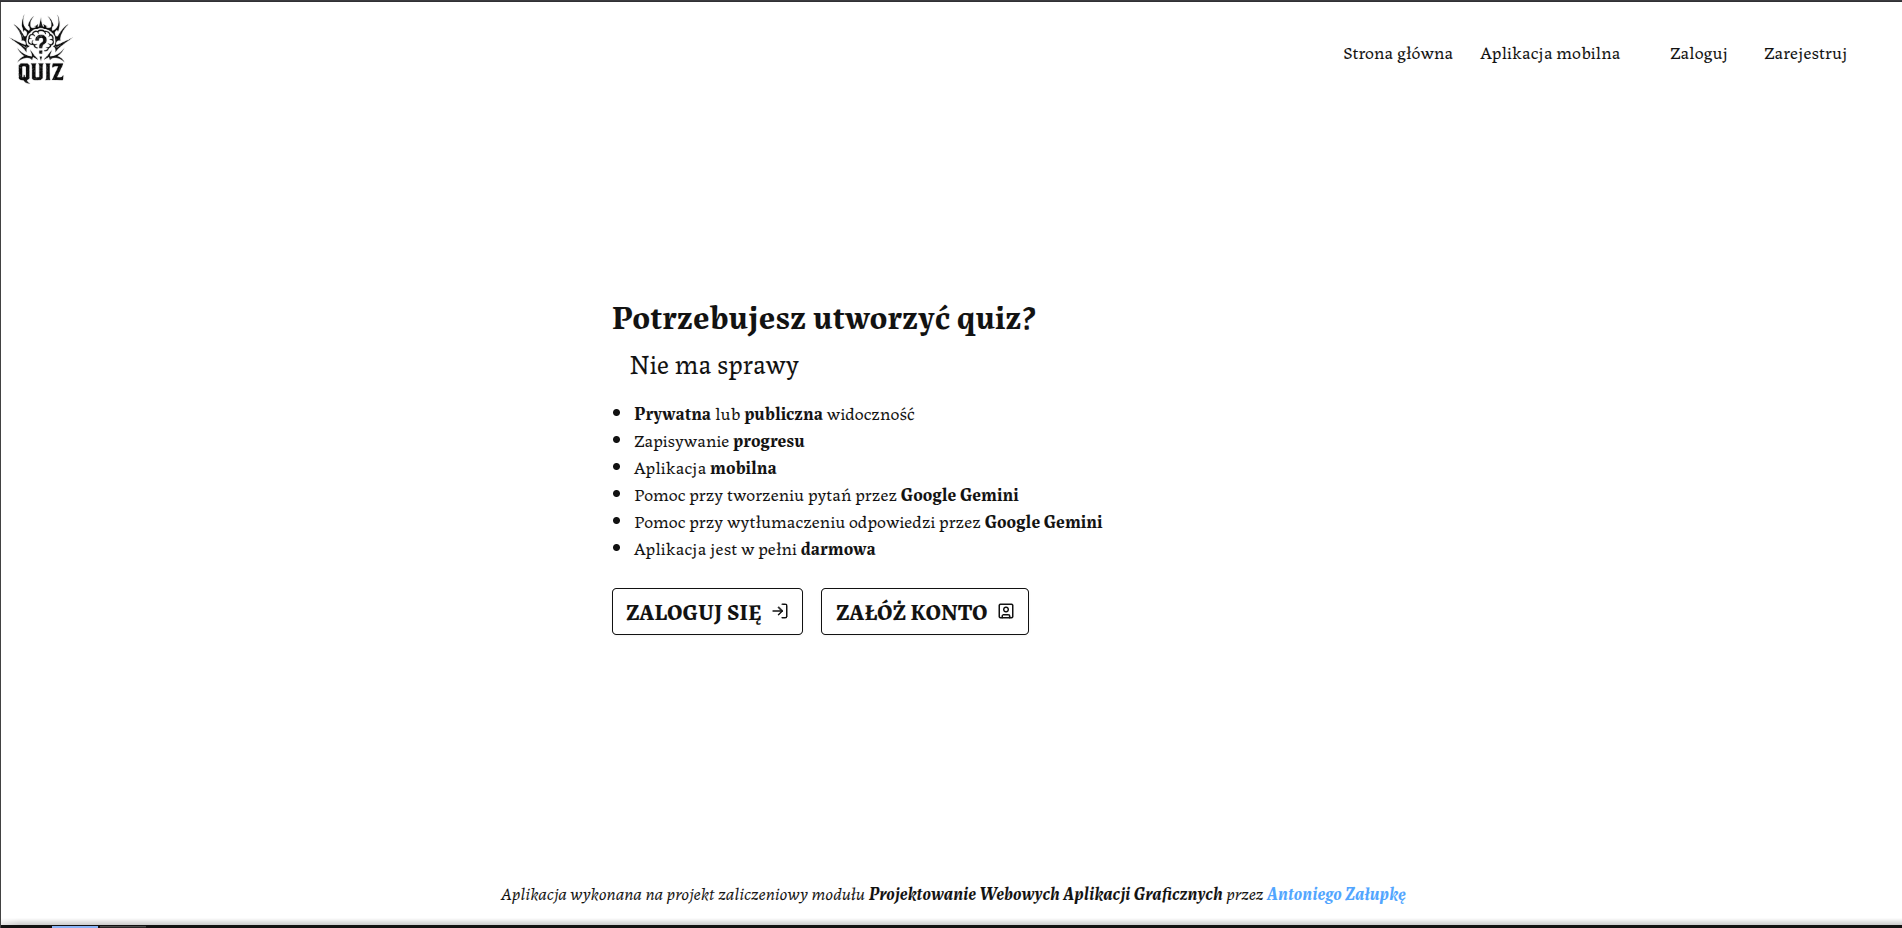
\includegraphics[width=0.5\textwidth]{../_assets/web/index.png}
            \caption{Strona główna przed zalogowaniem.}
            \label{fig:index}
          \end{figure}
        \end{minipage}

        \item Kreator quizu \\
        \begin{minipage}{0.4\textwidth}
          \begin{itemize}
            \item Możemy wygenerować quiz za pomocą modelu językowego Google Gemini.
          \end{itemize}
        \end{minipage}
        \begin{minipage}{0.6\textwidth}
          \begin{figure}[H]
            \centering
            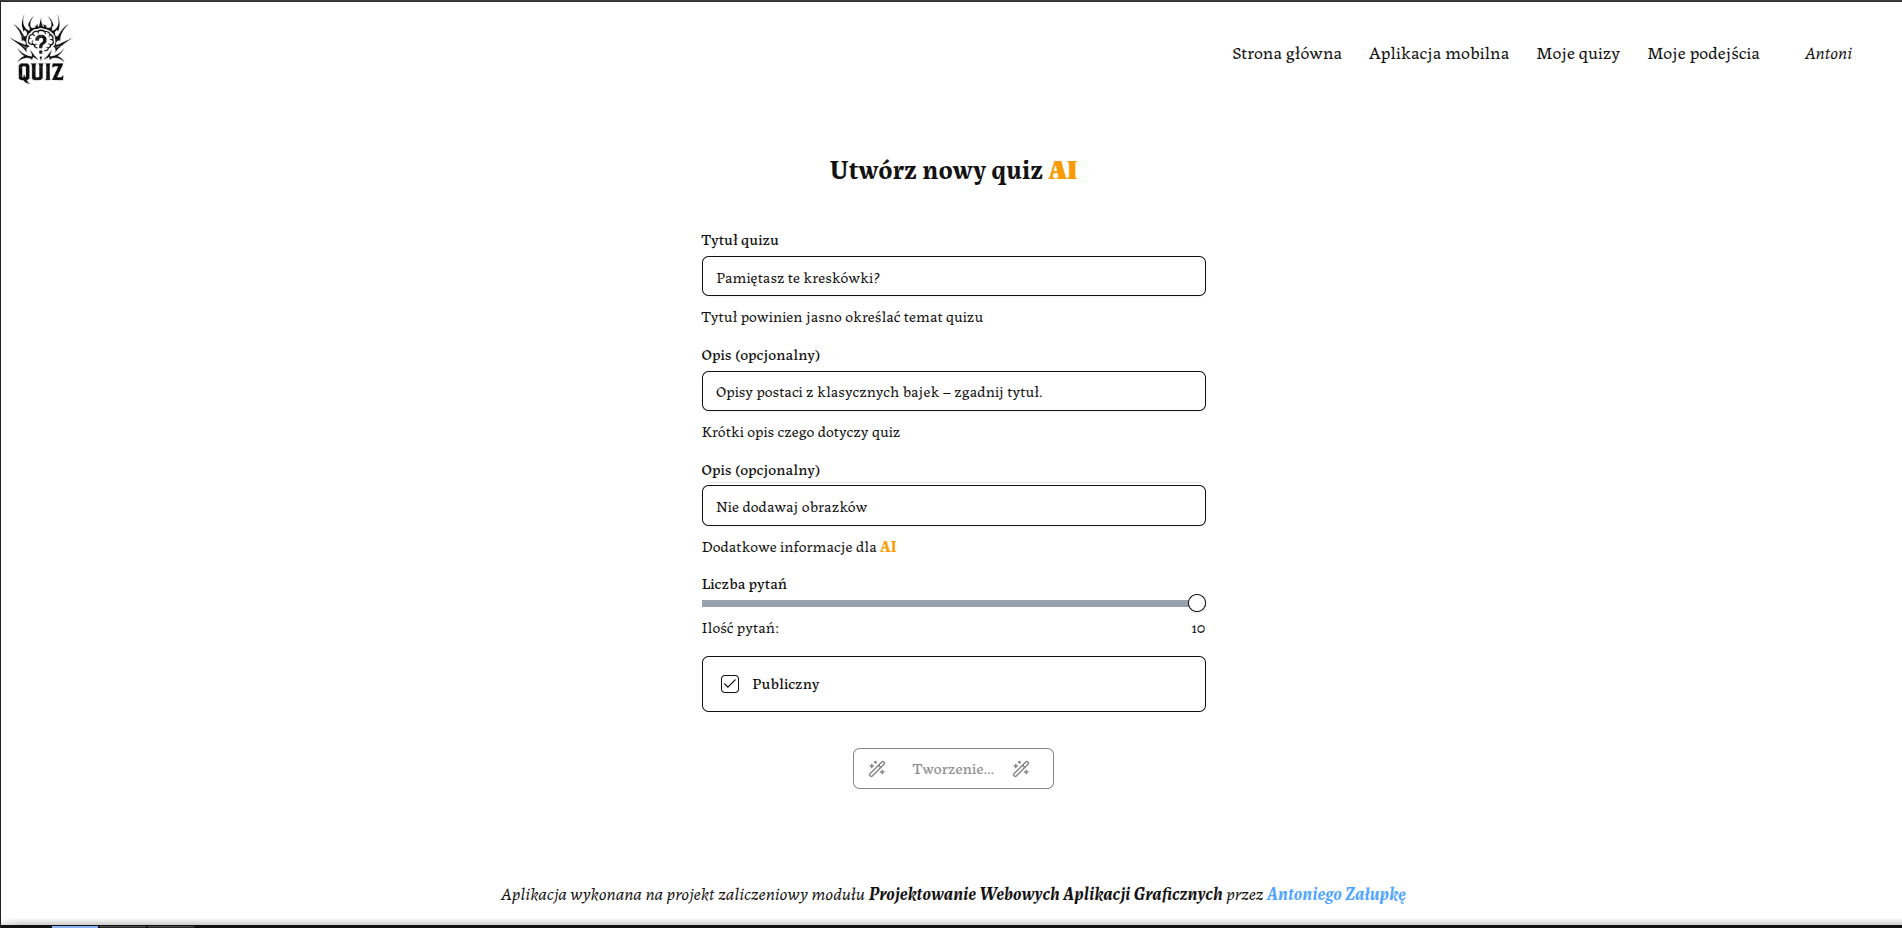
\includegraphics[width=0.5\textwidth]{../_assets/web/createAi.png}
            \caption{Automatyczny kreator tworzenia quizu.}
            \label{fig:createAi}
          \end{figure}
        \end{minipage}

		\item Edytor quizu \\
        \begin{minipage}{0.4\textwidth}
          \begin{itemize}
            \item Quiz możemy również stworzyć lub edytować ręcznie, korzystając z edytora JSON.
          \end{itemize}
        \end{minipage}
        \begin{minipage}{0.6\textwidth}
          \begin{figure}[H]
            \centering
            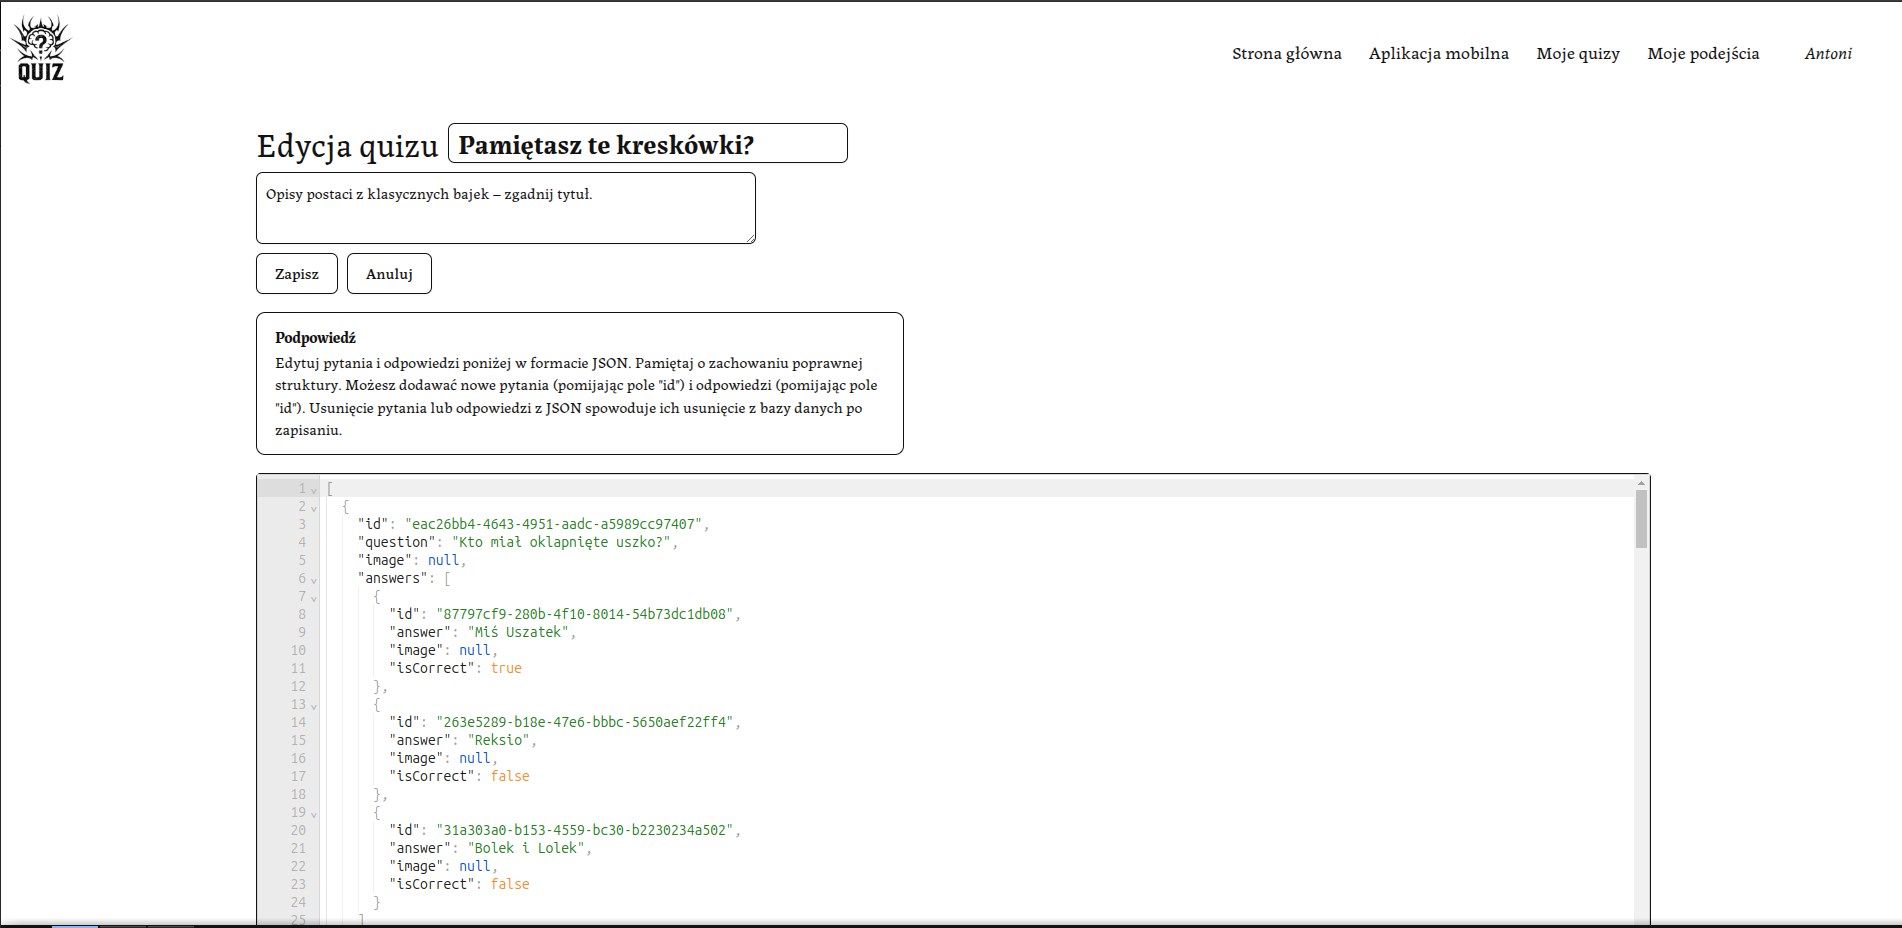
\includegraphics[width=0.5\textwidth]{../_assets/web/edit.png}
            \caption{Edytor quizu.}
            \label{fig:edit}
          \end{figure}
        \end{minipage}

		\item Lista quizów \\
        \begin{minipage}{0.4\textwidth}
          \begin{itemize}
            \item Możemy przeglądać listę quizów. Są tutaj widoczne nasze quizy i publiczne quizy innych użytkowników.
          \end{itemize}
        \end{minipage}
        \begin{minipage}{0.6\textwidth}
          \begin{figure}[H]
            \centering
            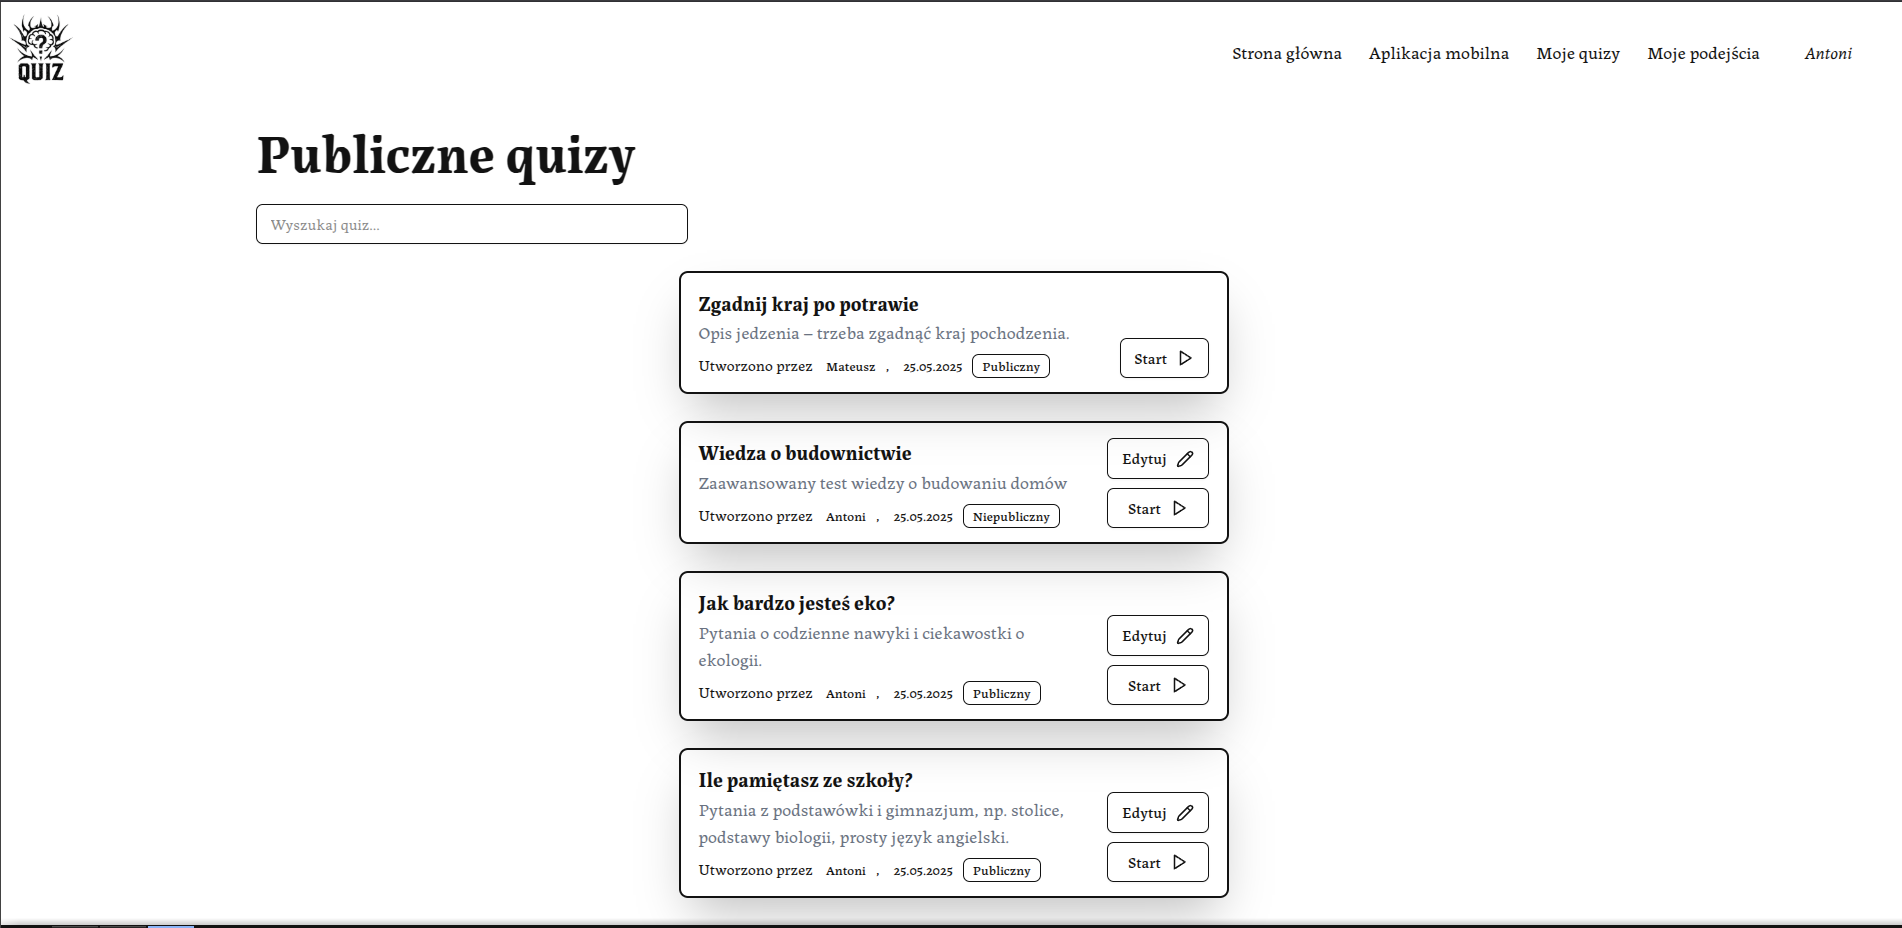
\includegraphics[width=0.5\textwidth]{../_assets/web/quizzes.png}
            \caption{Lista quizów (jest to też strona główna po zalogowaniu).}
            \label{fig:quizzes}
          \end{figure}
        \end{minipage}

		\item Podejście do quizu \\
        \begin{minipage}{0.4\textwidth}
          \begin{itemize}
            \item Rozpoczynając podejście wyświetlana jest lista pytań.
            \item Przy każdym pytaniu możemy sprawdzić poprawność odpowiedzi.
          \end{itemize}
        \end{minipage}
        \begin{minipage}{0.6\textwidth}
          \begin{figure}[H]
            \centering
            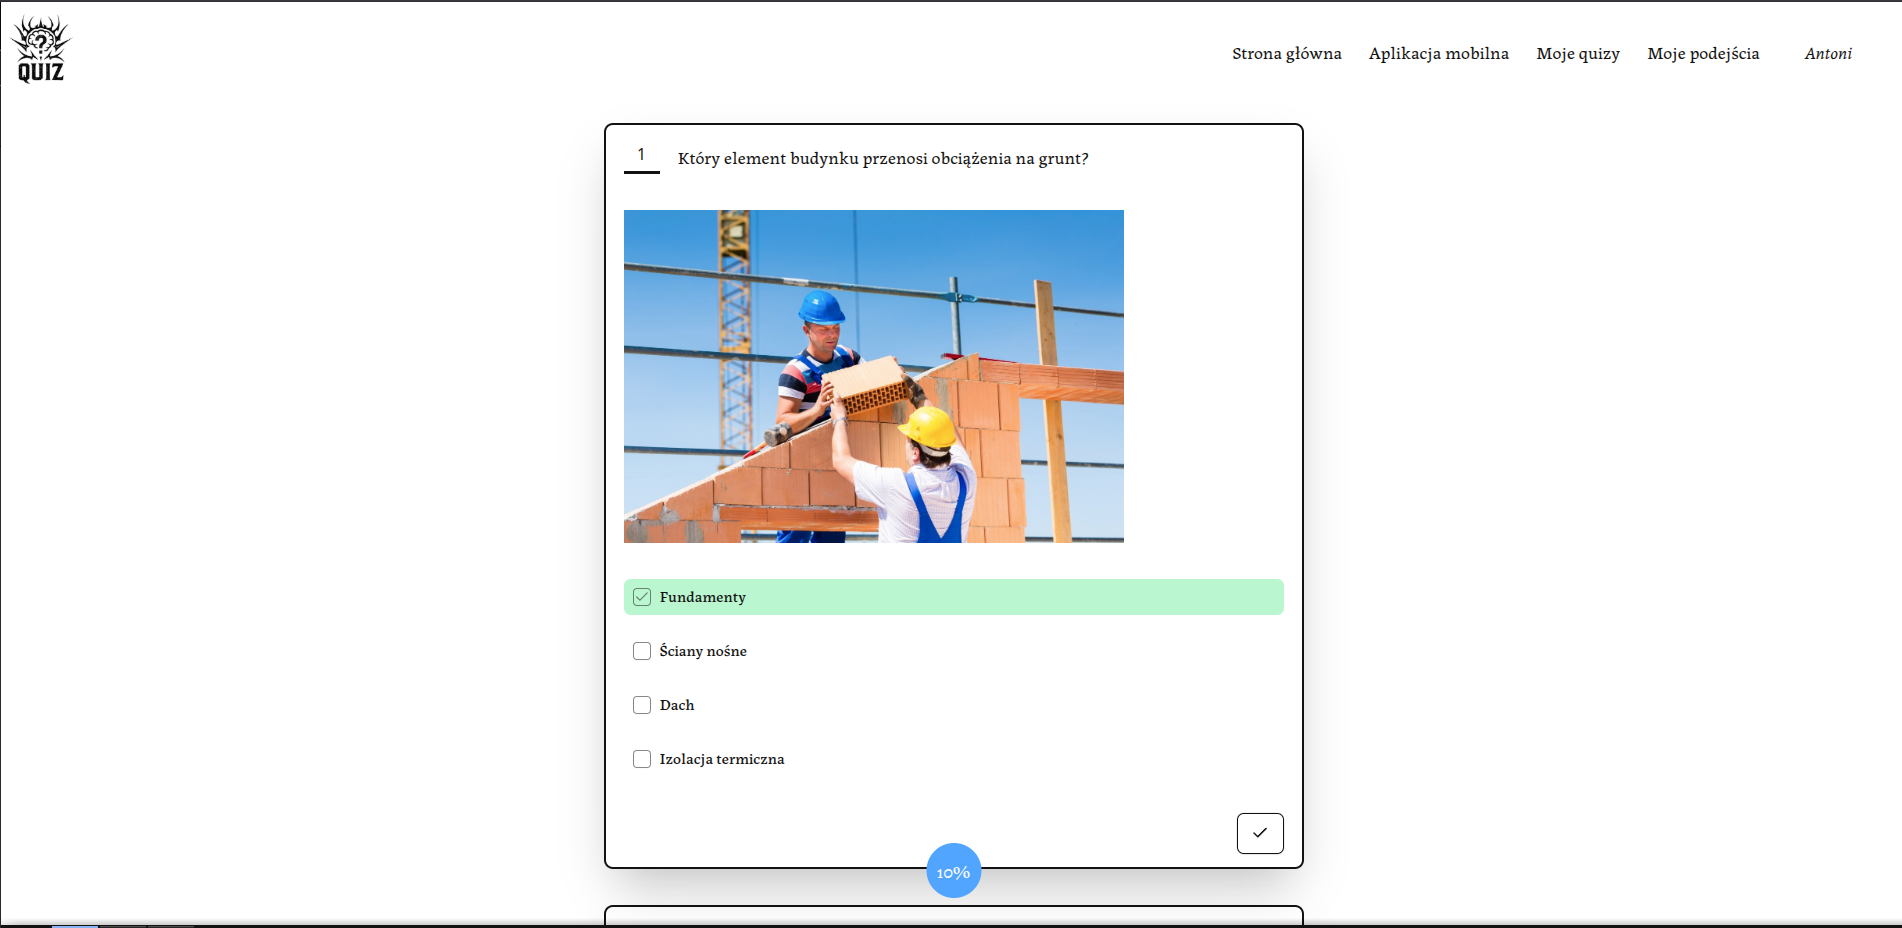
\includegraphics[width=0.5\textwidth]{../_assets/web/attempt.png}
            \caption{Podejście do quizu.}
            \label{fig:attempt}
          \end{figure}
        \end{minipage}

		\item Podsumowanie podejścia \\
        \begin{minipage}{0.4\textwidth}
          \begin{itemize}
            \item Przy każdym podejściu mamy możliwość sprawdzenia podsumowania.
            \item W podsumowaniu wyświetlane są podstawowe informacje o podejściu, takie jak czas trwania i liczba poprawnych odpowiedzi.
          \end{itemize}
        \end{minipage}
        \begin{minipage}{0.6\textwidth}
          \begin{figure}[H]
            \centering
            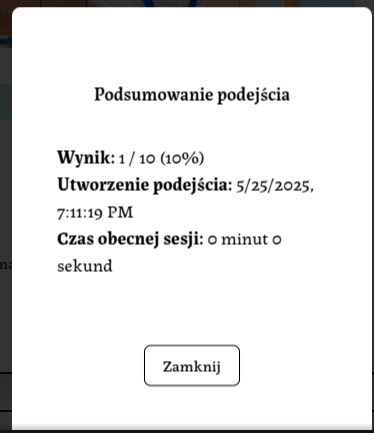
\includegraphics[width=0.5\textwidth]{../_assets/web/summary.png}
            \caption{Podsumowanie podejścia do quizu.}
            \label{fig:summary}
          \end{figure}
        \end{minipage}

      \end{enumerate}

    \section{Perspektywy rozwoju}
      Posiadam następujące pomysły na rozwój aplikacji w przyszłości:
      \begin{itemize}
        \item Optymalizacja backendu poprzez zapisywanie migawek podejść. Pozwoli to obliczać wynik na frontendzie bez utraty synchronizacji.
        \item Integracja z systemem rekomendacji quizów na podstawie historii użytkownika.
        \item Wprowadzenie trybu nauki z wykorzystaniem AI, który będzie sugerował pytania do nauki.
        \item Rozbudowa o tryb współpracy wielu graczy, gdzie użytkownicy mogą wspólnie rozwiązywać quizy.
        \item Implementacja powiadomień push dla nowych quizów i aktualizacji.
        \item Ulepszenie interfejsu użytkownika poprzez dodanie animacji i lepszej nawigacji.
      \end{itemize}

    \section{Wnioski}
        Przed rozpoczęciem projektu miałem doświadczenie w tworzeniu aplikacji webowych w bibliotece React.
        Projekt ten pokazał mi, że współcześnie Vue jest koncepcyjnie bardzo podobne do Reacta, a różnice znajdują się głównie w sposobie zarządzania stanem i strukturze komponentów.
        Poszerzyłem wiedzę o frameworku Vue oraz o architekturze aplikacji opartych na GraphQL.

\end{document}